\documentclass[12pt]{article}
\usepackage[utf8]{inputenc}
\usepackage[english,russian]{babel}
\usepackage[12pt]{extsizes}
\usepackage{booktabs}
\usepackage{graphicx}
\usepackage{graphicx,psfrag}
\usepackage{cite}
\usepackage{sectsty}
\usepackage{amsmath, esint, setspace, fancyhdr, amsfonts, bookmark, blindtext}

\graphicspath{{Figures/}}
\DeclareGraphicsExtensions{.pdf,.png,.jpg}
\setlength{\textheight}{8in}
\setlength{\textwidth}{6.6in}
\setlength{\headheight}{0in}
\setlength{\headsep}{0.2in}
\setlength{\topmargin}{0in}
\setlength{\oddsidemargin}{0in}
\setlength{\evensidemargin}{0in}
\setlength{\parindent}{.3in}
\renewcommand{\baselinestretch}{1.4}

\doublespacing

\begin{document}
\begin{titlepage}

\begin{center}
Санкт-Петербургский политехнический университет Петра Великого\\
Институт прикладной математики и механики\\
Кафедра прикладной математики\\
\hrulefill
\end{center}

\begin{flushleft}
\rule{9cm}{0pt} {Работа допущена к защите}\\
\rule{9cm}{0pt} Зав. кафедрой\\
\rule{9cm}{0pt} \rule{2.5cm}{0.5pt} {\bfseries{М. Е. Фролов }}\\
\rule{9cm}{0pt} "\rule{.9cm}{0.5pt}" \rule{4cm}{0.5pt}
\end{flushleft}

\vspace{1.5cm}

\begin{center}
{\large {\bfseries ОТЧЕТ\\
о научно-исследовательской работе}}\\

\bigskip \bfseries{Тема:} {\bfseries \emph{Классификация саженцев растений}}
\end{center}

\vspace{1.cm}

\begin{flushleft}
Направление: 01.03.02 Прикладная математика и информатика

\vspace{1.cm}

Выполнил студент гр. 33631/4 \hfill{Камалетдинова Ю.А.} \\ 

\vspace{0.2cm} Руководитель \hfill{Яковлев Д.В.}

\end{flushleft}

\vspace{1.5cm}

\begin{center}
Санкт-Петербург\\
2019
\end{center}

\end{titlepage}


\tableofcontents
\addtocontents{toc}{~\hfill\par}
\vfill ~
\setcounter{section}{0}

\section{Введение}

\indent{\indent Потребность в сельскохозяйственных продуктах увеличивается с каждым днем, как и растет население планеты Земля. Часть работ выполняют люди, и силы уходят на контроль качества выращиваемых культур. Мы сможем использовать временные и природные ресурсы более бережно и экономно, увеличим урожаи, если научимся дифференцировать благородные культуры и отличать их от сорняков без помощи человека. }

\indent{ В такой ситуации естественным образом приходит мысль об автоматизации процессов, например, классификация саженцев по фотоснимкам. Возникает мысль задействовать нейросети, что обосновано преимуществами, но также они обладают недостатками в виде вычислительных затрат. }

\indent{  Возможно использовать алгоритмы другой группы, но они требуют более тонкой настройки для достижения сопоставимого результата, а иногда вовсе не могут быть улучшены. В данной работе поставим задачу классификации растений и решим ее методом опорных векторов. }

\section{Анализ набора данных}
\subsection{Первичный взгляд на данные}

\indent{\indentИсследуемый набор данных был собран группой Орхусского университета по обработке сигналов в сотрудничестве в Университетом Южной Дании. Этапы создания коллекции описаны с статье \cite{bib_1}. Набор содержит приблизительно 960 уникальных изображений растений 12 видов, находящихся на разных стадиях роста. }\\
\indent{Изучимы исходные данные. Построим образцы каждого класса в виде сетки}

\begin{figure}[h]
	\centering
	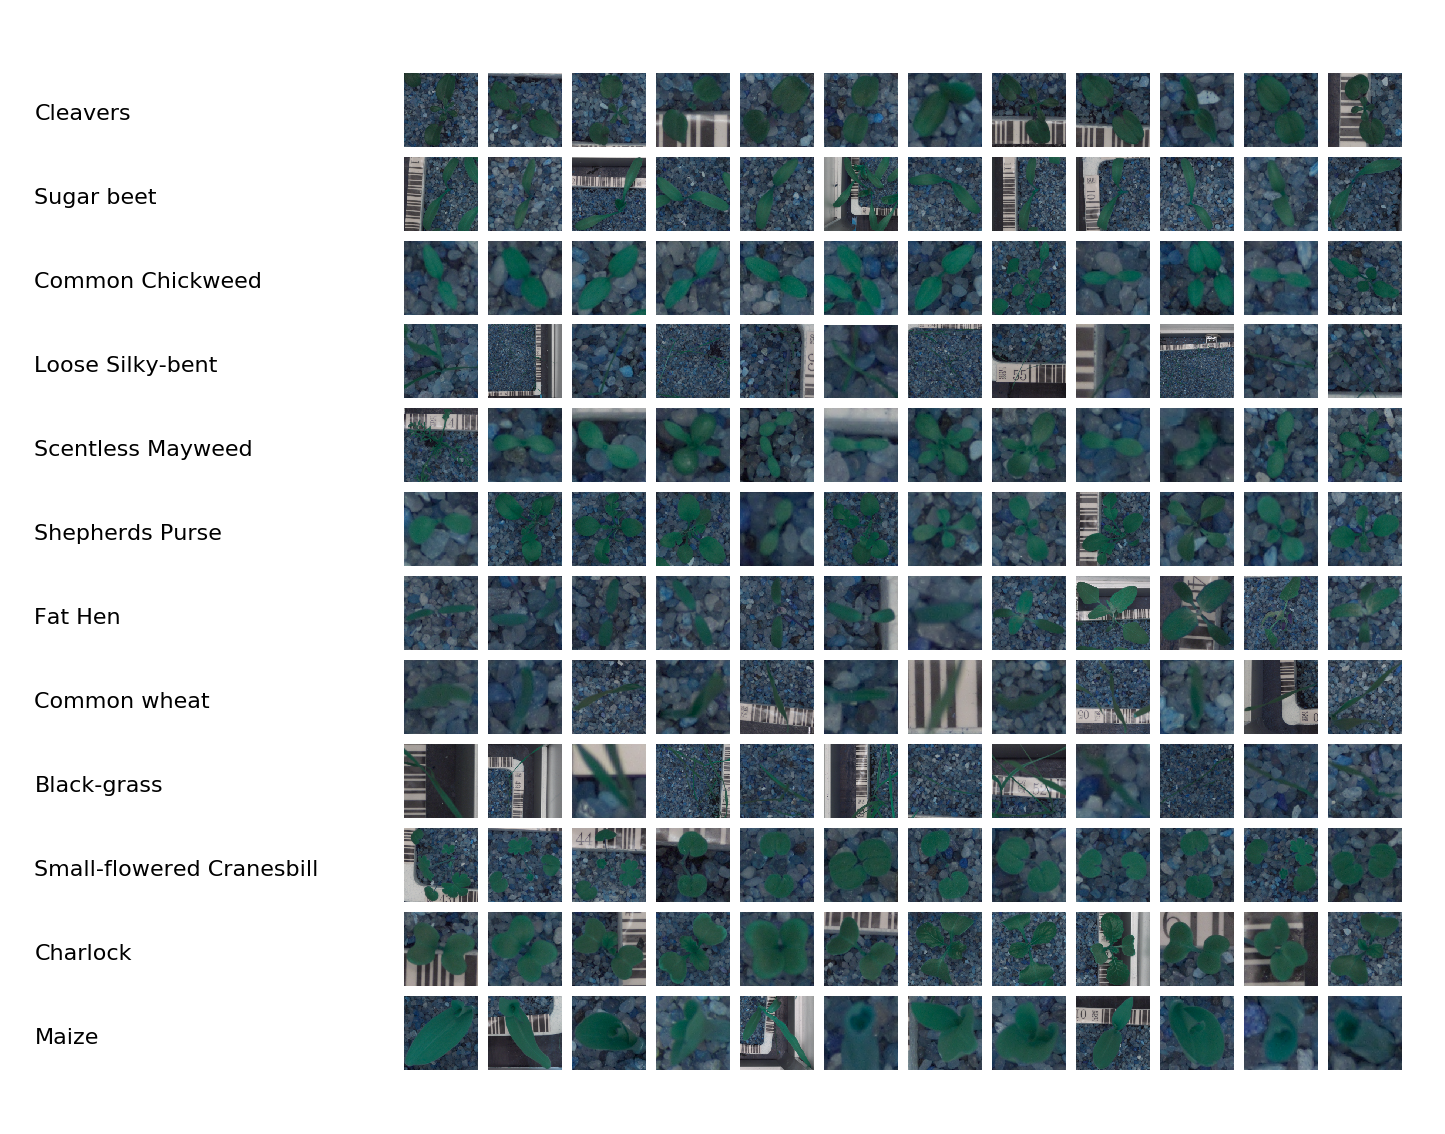
\includegraphics[width=16.cm, height=12.cm]{first_view_grid_1}
	\caption{Образцы растений каждого вида (построчно)}
	\label{fig_1}
\end{figure}

\indent{ Проанализировав снимки, можно сделать некоторые выводы:}
\begin{itemize}
	\item {Исходные изображения уже кадрированы и не требуют дополнительной обрезки 
	\begin{figure}[h!]
		\centering
		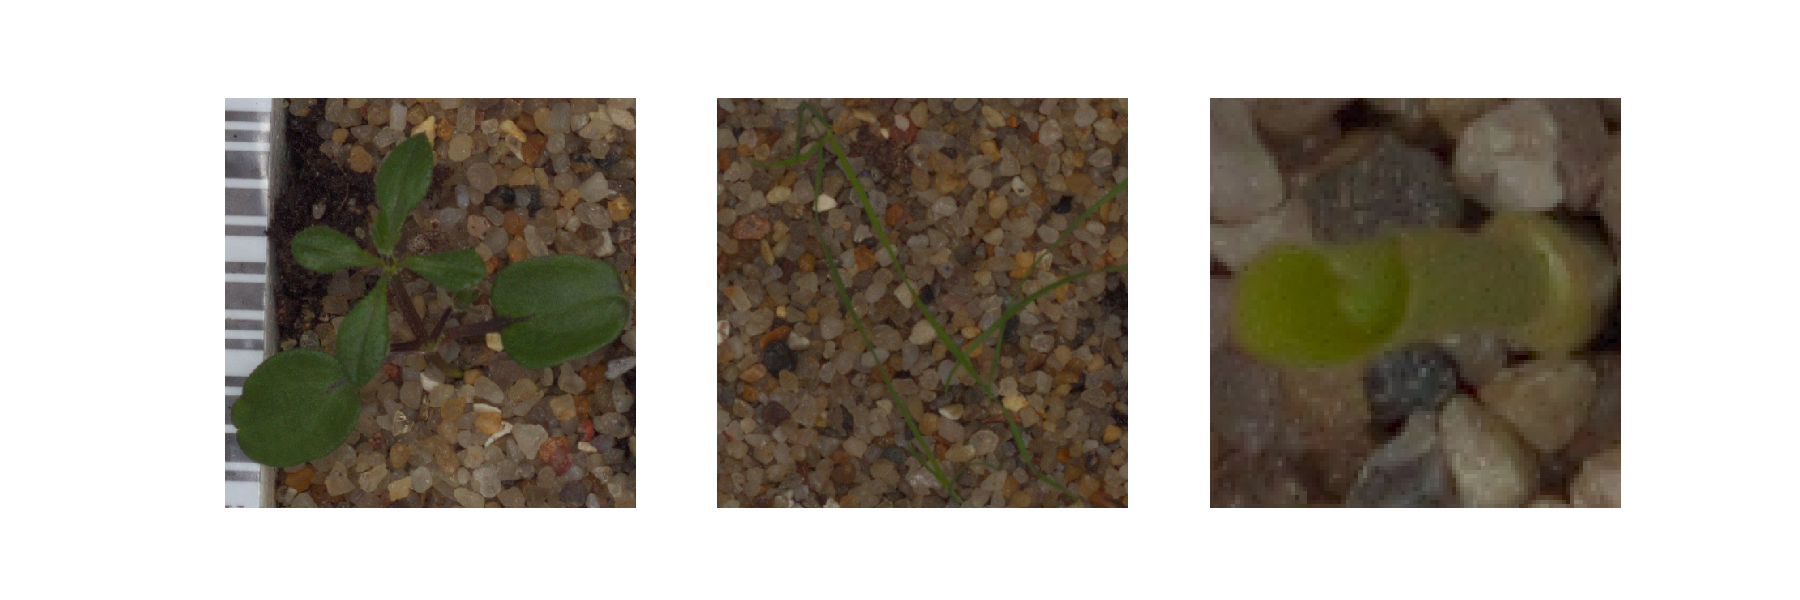
\includegraphics[width=15.cm, height=5.cm]{first_view_three_1}
		\caption{Примеры исходных изображений}
		\label{fig_2}
	\end{figure}
	}
	\item Разрешения изображений варьируются от 50х50px до 2000х2000px, поэтому необходимо привести весь набор к единому разрешению. 
	\item Фон на снимках различен, необходимо выбрать спосбо сегментации, наиболее подходящий для большинства
\end{itemize}

\indent{Заметим, что все представленные растения окрашены в зеленый цвет. Поэтому мы можем создать маску, фильтрующую диапазон зеленых оттенков и удаляющую пиксели остальных цветов. Для реализации воспользуемся библиотекой компьютерного зрения OpenCV \cite{bib_2} и библиотекой для вычислений Numpy \cite{bib_3} языка программирования Python.}

\subsection{Загрузка изображений}

\indent{\indent Библиотека OpenCV использует цветовую модель BGR (Blue Green Red) для представления цветных изображений. Каждый пиксель характеризуется составляющими синей, зеленой и красной компонентами. Загрузив изображение, изменим его разрешение до 200х200px.}

\subsection{Маскирование}

\indent{\indent Воспользуемся цветовой моделью HSV (Hue Saturation Value) \ref{fig_3}. В формате BGR значение каждой компоненты зависит от количества света, попадающего на объект. HSV же позволяет разграничить информацию о цвете и яркости. Оттенок, насыщенность и интенсивность позволят задать нижнюю и верхнюю границы оттенков некоторого цвета, в данном случае –– зеленого.}
\begin{figure}[h]
	\centering
	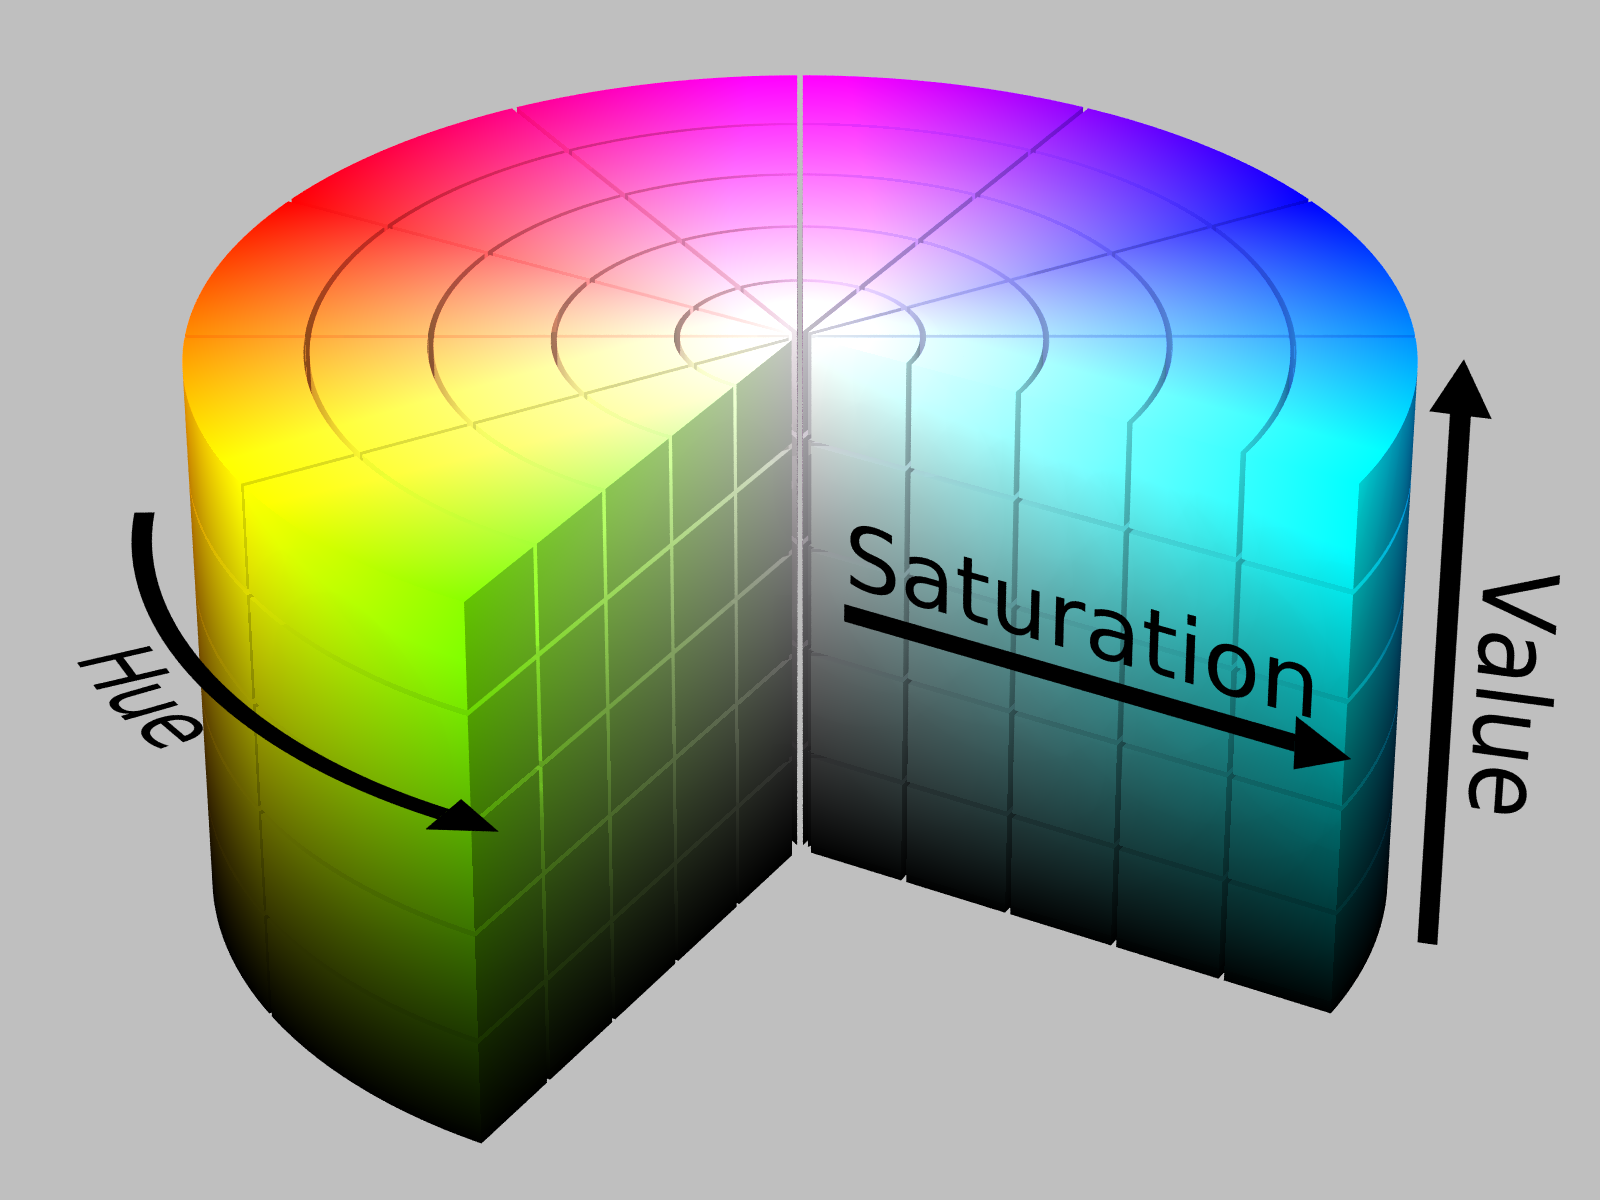
\includegraphics[width=9.cm, height=7.cm]{hsv}
	\caption{Цветовая модель HSV}
	\label{fig_3}
\end{figure}

\begin{figure}[h]
	\centering
	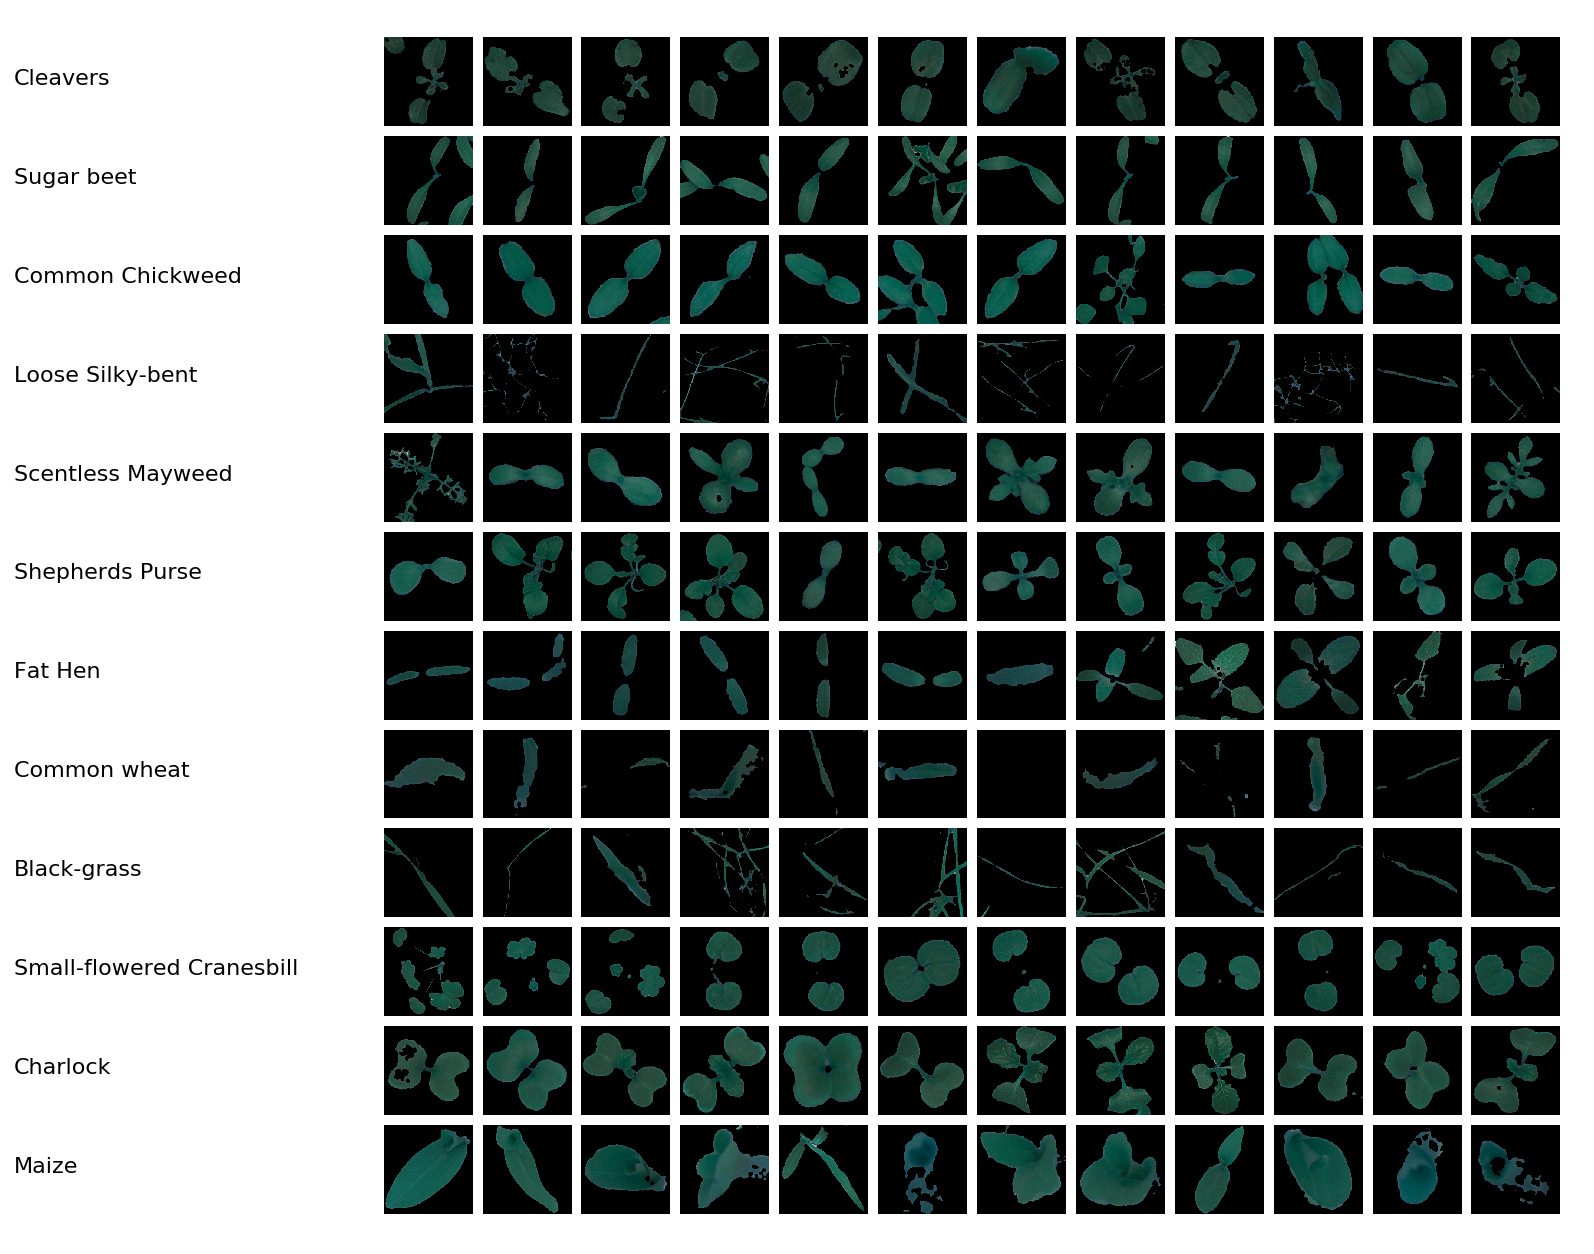
\includegraphics[width=16.cm, height=12.cm]{segmented_part_1}
	\caption{Образцы растений каждого вида после сегментации (построчно)}
	\label{fig_4}
\end{figure}


\section{Извлечение признаков}

\section{Результаты исследований}

\section{Вывод}

\newpage

\begin{thebibliography}{}
	\bibitem{bib_1} Giselsson, T., Jørgensen, R., Jensen, P., Dyrmann, M., and Midtiby, H. (2017). A Public Image Database for Benchmark of Plant Seedling Classification Algorithms. 
	\bibitem{bib_2} Bradski, G. (2000). The OpenCV Library. Dr. Dobb's Journal of Software Tools.
	\bibitem{bib_3} Oliphant, T. E. (2006). A guide to NumPy (Vol. 1). Trelgol Publishing USA.
\end{thebibliography}

\end{document}{}